\documentclass{article}

\usepackage{biblatex}
\usepackage{amsmath}
\usepackage{graphicx}
\usepackage{subfig}
\addbibresource{references.bib}
\usepackage{float}

\title{Applying Regression Test Selection on the example of Business Central}
\author{Diego Joshua Martinez Pineda (diem@itu.dk)\\Supervisor: Mahsa Varshosaz (mahv@itu.dk)}

\begin{document}
\maketitle

\begin{abstract}
In this research project, we address the problem of implementing a test selection algorithm on the Business Central project. For the scope of this project, a single test selection algorithm was implemented, which is based on test coverage information. The findings of this work should serve as a foundation to explore the different selection and prioritizations techniques in this system. Much of the work presented here went into understanding the context and setting of the system, sufficiently to execute the algorithm in actual revision examples. The insights acquired provide a basis for future evaluation settings to increase the validity of the results here presented and of future algorithms to be evaluated.
\end{abstract}

\section{Introduction}
\subsection{The test selection problem}
   When working with large software systems, regression testing is a valuable technique that increases the confidence of the product stakeholders that future revisions, new features, and evolution of the system will not break previous functionality.

   For this reason, it is common for products to have the execution of the regression test suite as part of the main pipeline of the product. However, when systems are sufficiently large, it becomes very expensive to run the full suite of tests.

   A test selection algorithm aims at choosing a subset of a full test suite to run, that is not as expensive as running all tests cases. However, this selection must preserve the capabilities of fault detection that the full test suite has. This means that careful selection must be made so that the confidence in fault detection is not lost because of not selecting some test cases.

\subsection{Business Central}
   Business Central is an ERP software system from Microsoft, it is a large software system, with different sets of tests for the diverse aspects of the product.

   For the test selection explored in this project, the test suite of the application code (business logic) is explored. The business logic of the system is written on AL, a DSL similar to Pascal that has primitives for interacting with the runtime of Business Central.

\section{Test Selection Method}
\subsection{Overview}\label{section:overview}

The idea for the method explored in this research project is to use the line coverage information that each test case produces, and ``read it backward'' when given a code change in those lines. That means that by looking at which lines were modified on a given change, given that we know which tests were affecting those particular lines then we know that we should select those tests.

To further illustrate, see for example figure \ref{fig:diff}. Here we can see a \texttt{diff} of an AL code file on a given revision that added lines in between what previously were lines 30-31, and 39-40. Also what was previously line 29 was removed. Therefore, provided that we know which tests were hitting those lines, then we could propose them as tests to be selected.

\begin{figure}[H]
  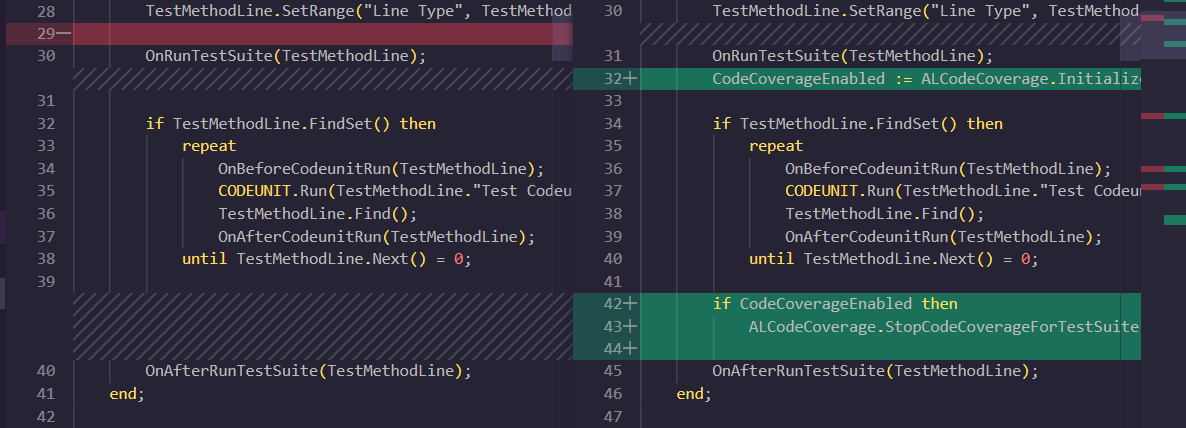
\includegraphics[width=\textwidth]{images/diff.png}
  \caption{A revision change on AL code.}
  \label{fig:diff}
\end{figure}

Intuitively, this seems like a good heuristic to select tests. However, we do not claim it is sufficient, furthermore, examples can be shown where this heuristic fails. For example, when a part of the code is dependent on the side effects it produces; then changing the environment of it through the side effects of a revision, can cause a seemingly unrelated set of test cases to fail.

This method is meant to provide a foundation for further explorations on selection methods using different criteria besides this straightforward heuristic. We describe the different ways we can extend this method on section \ref{section:future-work}.
\subsection{AL background information}\label{section:al-background-info}
Before explaining details of the work done, we present for reference and clarity some of the minimal background knowledge required to understand how code and tests in AL are defined.

As mentioned in the introduction, AL is a DSL for this specific system and extensions for this system. The code is organized in several \emph{AL objects}, which do not resemble objects in the traditional OOP sense, but objects from the system runtime. \emph{AL objects} can be from different types, for example:
\begin{itemize}
\item \emph{Tables}. Corresponding to underlying SQL Server tables.
\item \emph{Pages}. Corresponding to interactive pages the user can see.
\item \emph{Codeunits}. Modules with \emph{procedures}, that is code that can be reused throughout the codebase
\end{itemize}

Each AL file in the codebase has as part of its definition, the type of object it is. Also relevant to its definition is the usage of numeric IDs to identify the AL Objects. Each ID must be unique throughout the instance of the system containing it for such object type.

To make things more concrete, figure \ref{fig:al-examples} shows an example of AL objects of types \emph{page} and \emph{table}. They are identified by both the type of object and ID, notice in this example, they share the same id, but they differ on the type of object.
\begin{figure}[H]
  \centering
  \subfloat[\centering AL Page]{{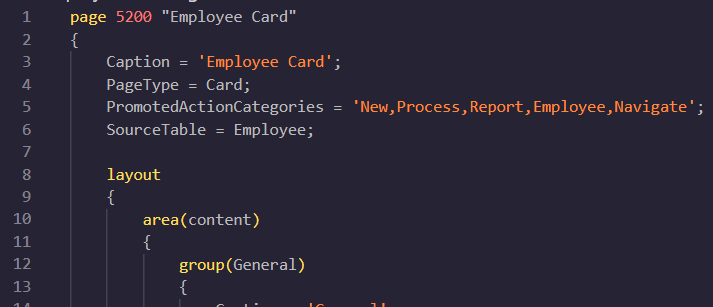
\includegraphics[width=5.5cm]{images/alpage.png} }}
  \qquad
  \subfloat[\centering AL Table]{{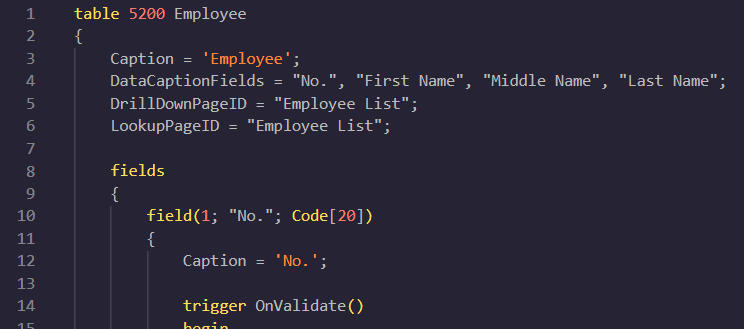
\includegraphics[width=5.5cm]{images/altable.png} }}
  \caption{Examples of \emph{AL Objects}. }
  \label{fig:al-examples}
\end{figure}

A mechanism for code reuse in this language is, as listed above, \emph{codeunits}, which is similar to the concept of ``modules'' in other languages. They consist of several \emph{procedures}. See an example in figure \ref{fig:codeunit-example}
\begin{figure}[H]
  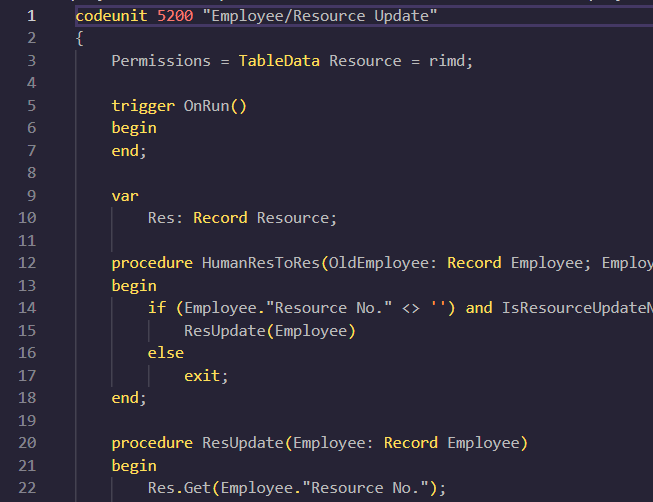
\includegraphics[width=\textwidth]{images/alcodeunit.png}
  \caption{Example of an \emph{AL Codeunit} with procedures \texttt{HumanResToRes} and \texttt{ResUpdate}.}
  \label{fig:codeunit-example}
\end{figure}

Finally, we explain how scenario tests for AL code are defined. Unit and scenario tests for application code are written in AL themselves, they correspond to \emph{codeunits} that are marked as tests. Procedures within such a \emph{test codeunit} may correspond to scenarios to be tested. See figure \ref{fig:al-test-examples} for an example on how \emph{codeunits} are marked as tests and a scenario example.

\begin{figure}[H]
  \centering
  \subfloat[\centering AL Test Codeunit Definition]{{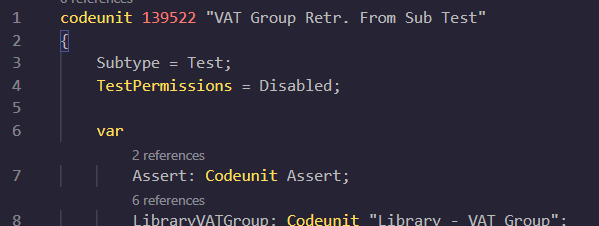
\includegraphics[width=5.5cm]{images/altestcodeunit.png} }}
  \qquad
  \subfloat[\centering AL Test Procedure - Scenario]{{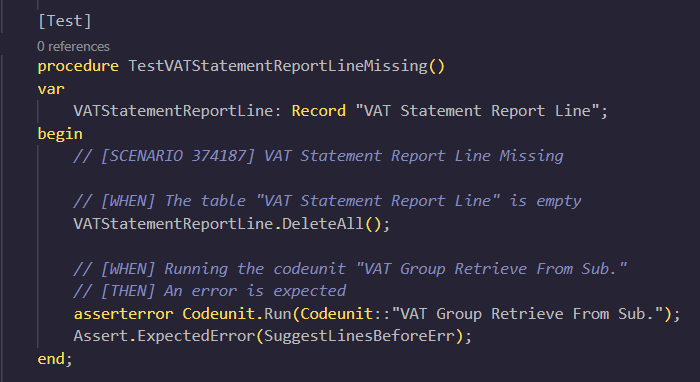
\includegraphics[width=5.5cm]{images/altestscenario.png} }}
  \caption{Examples of definition of AL Test Scenarios. }
  \label{fig:al-test-examples}
\end{figure}


\subsection{Coverage information of test runs on AL}\label{section:cov-info}
AL provides primitives to record line coverage information when executing arbitrary sections of code. This line coverage information has the following components, relevant for the selection method:
\begin{itemize}
\item Object ID
\item Object type
\item Line number
\item Number of hits
\end{itemize}

As explained in section \ref{section:al-background-info}, \emph{Object ID} and \emph{Object Type} are properties related to the way the code is organized in this language. Both the \emph{Object ID} and \emph{Object Type} identify a file in the codebase, for which the related line number refers to.

It is relevant to stress that this information does not provide a file path on the codebase directly, but only a mean for identification.

Currently on the system, this primitive is used throughout the execution of the test suite. These measures test coverage information, providing the set of objects and lines covered by the suite, and it is used to impose coverage requirements for new additions to the codebase.

This means, that the information obtained by recording coverage throughout the complete execution of the test suite, does not distinguish between different test cases. The coverage information currently available on each run does not have which lines were hit by a particular test, but it only determines that it was hit by some test on the test suite.

However, previously in section \ref{section:overview}, we described the method as selecting those test cases which affected a particular set of lines. With the current test coverage information, it is not possible to make that distinction.

For this reason, changes on the test runner were needed, to allow for individual tracking of coverage information per test case. However, these changes are currently not on the main pipeline of the product \footnote{These changes were not work of the author, but from Nikola Kukrika nikolak@microsoft.com, as they are on the backlog to be added to the pipeline}.

Another relevant technical consideration of how this information was dealt with, is how the output of the coverage information of each test case was stored. This was part of the work for this project. An SQLite database was proposed to allow for querying the information in different ways efficiently. The current usage of this information within the product is in form of CSV files, so the corresponding parsing-loading scripts were therefore in the scope of the project as well.

Figure \ref{fig:erdiagram} shows the proposed ER diagram in crow's foot notation of the DB schema proposed. AL Objects are modeled with their lines in a one-to-many relationship. These in turn are joined through the \texttt{coverage data} pivot table with the test procedures.
\begin{figure}[H]
  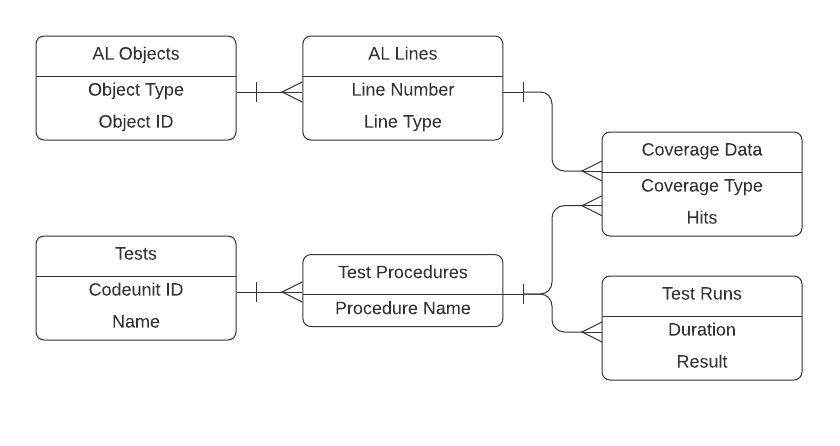
\includegraphics[width=\textwidth]{images/erdiagram.png}
  \caption{Proposed ER diagram for the coverage database schema}\label{fig:erdiagram}
\end{figure}

\subsection{Representing revision differences}\label{section:rev-diffs}

The codebase with the business logic is composed of several AL applications.

When working on a new revision, some of the files on these applications get changed, removed or added. The canonical way of treating with differences between revisions is with line \texttt{diff}s of the files, see for example figure \ref{fig:diff}.

The output information of such \texttt{diff} is the set of file paths added, removed, or changed, together with the lines where these changes occured.

However, in the previous section we explained that the coverage information we are able to extract has as component the Object Id and Object Type where line coverage was recorded. While this properties correspond uniquely to a file in the codebase, it is not a direct inspection of the file path where code was changed that will tell us the information of which Object Id and Object Type that file has.

Even more, we are considering changes on the whole codebase and that may imply changes on tests as well, for example adding new test procedures. For these kind of changes we would not like to have the same interpretation on tests that should be selected, we would like for example that whenever test procedures get added, that they are at least selected. This would not be possible by only restricting to coverage information since these tests did not exist previously.

These two situations give way to thinking that more information than just the file path and lines changed is required from a given revision change. For this selection method, a lightweight parsing was performed on the given changed files to extract which Object Id is being affected, and whether or not such object corresponds to a test.

Notice that the choice of what information to extract from a given revision change was just to address these two situations. We could however extract more information, enhancing our knowledge of what kind of change the revision affected; this could be even more granular for example to detect changes on specific procedures, addition of procedures, definition of new columns on a table; and in general, information more semantically related to the nature of the change. This could be a direction for future work, as input for more complex selection criteria. This is further explained in section \ref{section:future-work}.

For completeness, table \ref{table:revision-changes} shows the information extracted for identifying a set of revision changes. 

\begin{table}[h!]
\centering
\begin{tabular}{||c c||} 
 \hline
 Type of change & Parameters \\
 \hline\hline
 \texttt{AddObject} & None\\
 \texttt{DeleteObject} & \texttt{removedObjectId} \\
 \texttt{AddLinesObject} & \texttt{objectId}, \texttt{afterLine} \\
 \texttt{RemoveLinesObject} & \texttt{objectId}, \texttt{firstLineRemoved}, \texttt{nLinesRemoved} \\
 \texttt{AddTestObject} & \texttt{testCodeunitId} \\
 \texttt{DeleteTestObject} & \texttt{testCodeunitId} \\
 \texttt{AddLinesTestObject} & \texttt{testCodeunitId} \\
 \texttt{RemoveLinesTestObject} & \texttt{testCodeunitId} \\
 \hline
\end{tabular}
\caption{Information extracted from revision changes}
\label{table:revision-changes}
\end{table}

The code for obtaining such representation was as well part of this project. For reference, this consisted in taking the \texttt{diff} from the change, visiting each file on the appropriate revision, and parsing to obtain the required information.

\subsection{Test selection}\label{section:test-selection}

Given that coverage information per test procedure is available, and revision changes can be understood in terms of what the coverage information provides; we can specify the heuristic explained in section \ref{section:overview} by describing what tests should the algorithm select for each kind of revision change we observe. This is the main core procedure proposed for selecting tests on this project.

\subsubsection{Adding lines to an AL object}
Whenever lines are added to an AL object, they are added after a given line. The selected tests then are those that were hitting that line and the next.

For further illustration see figure \ref{fig:addinglinechange}, where we can see such a change, a new line was added between what previously was line 1107 and 1108. From the coverage information we can obtain the set of test procedures that on the previous revision were hitting those lines; this method selects those tests.

\begin{figure}[H]
  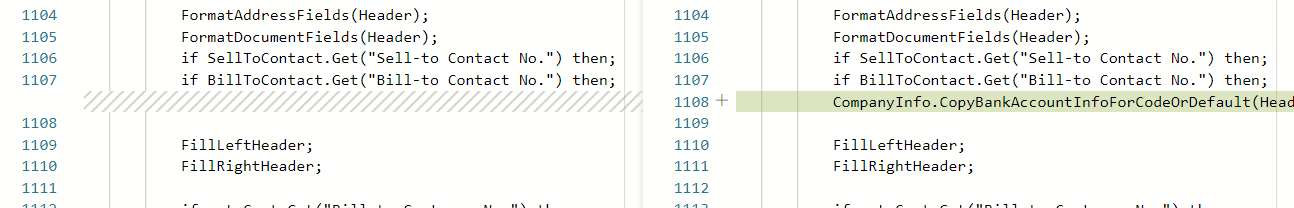
\includegraphics[width=\textwidth]{images/addinglinechange.png}
  \caption{Example of a change that added a line between what previously was line 1107 and 1108.}\label{fig:erdiagram}
  \label{fig:addinglinechange}
\end{figure}

\subsubsection{Removing lines from an AL object}
For removed lines, any test that was hitting what were previously those lines are selected.
\subsubsection{Adding an AL object}
We can not infer any test run from a new object, since coverage information would not include it.
\subsubsection{Removing an AL object}
We can understand this case as being the same as removing all the lines of it. Therefore any test hitting that object should be selected. It is worth noticing that this is not a traditional revision change, but it is taken into consideration for completeness.
\subsubsection{Adding lines to an AL test codeunit}
The current representation for the revision change does not distinguish if the lines added are because of adding new test cases on a given test codeunit, or because of changing a test procedure. Both cases could be treated differently if the model for the revision change allowed for that.

Instead, we only keep the information of to which test codeunit lines were added. As a conservative approach, in this method we select all test procedures inside this test codeunit.
\subsubsection{Removing lines from an AL test codeunit}
In the same vein as adding lines to an AL test codeunit, as a conservative measure, all test in this test procedure are selected.
\subsubsection{Adding an AL test codeunit}
For this case, we would like to select all the test procedures in the new test codeunit.
\subsubsection{Removing an AL test codeunit}
When removing a test codeunit, we can not infer running any test. However the Object Id of the removed test codeunit is kept, to filter our selection by removing any references to such tests.
\subsection{The full algorithm}
To wrap up the different parts of the selection method explained on the previous section, we give an overview of how these parts compose together.

A codebase at a given point in time can be enriched when running the test suite with the information of the lines covered by each test case. This is achieved through the modifications on the \emph{Test Runner} application explained on section \ref{section:cov-info}. This information is stored in a coverage database.

When a revision is given, we know the set of file paths and lines changed for such. We can leverage from parsing such files on each revision to gather more information about what this revision change implies. The information extracted is to allow for different test selection criteria for each type of change, as it is listed in section \ref{section:rev-diffs}, table \ref{table:revision-changes}. More generally, we can think of this step as extracting a helpful representation from the revision change.

With this information, the test selection criteria described in section \ref{section:test-selection} is then applied, resulting on a set of selected test cases.

Figure \ref{fig:testselection} shows an informal diagram to further illustrate the description here given.
\begin{figure}[H]
  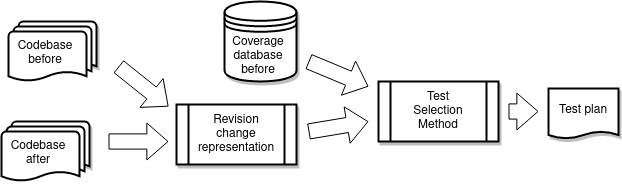
\includegraphics[width=\textwidth]{images/testselection.png}
  \caption{Informal diagram of the procedure for test selection.}
  \label{fig:testselection}
\end{figure}

\section{Evaluation}\label{section:evaluation}
\subsection{Metrics}
In the literature for the problem of test selection, several metrics have been proposed to quantify the different aspects addressed by a selection algorithm.

For instance, measuring how big is a given selection relates to the expected performance gains of using a method. After all, choosing all tests is a valid selection algorithm, although not ideal for our goal.

Another example is measuring how effective the algorithm was to select the faulty test cases. If our selection is very small it would be efficient, but if such selection is not capturing the faulty tests, then it is damaging to the product quality.

The metrics choosed were taken from a survey done by Pan, Bagherzadeh, et. al. in \cite{Pan2021TestCS}. One of the research questions they dealt with, was the metrics used to evaluate the TSP. Additionally other common metrics were used.
\subsubsection{Test selection execution time}
This metric measures the total time of running the selected subset of tests, against the total time that it takes to run all of them.

Ideally we would like this value to be as small as possible.
\subsubsection{Test selection time to first failure}\label{section:tffailure}
This metric measures the time taken for test execution until the first failure is detected, according to the proposed plan; with respect to the total execution time of all of them. Strictly speaking, this is a metric for evaluating a test prioritization technique, since a selection may have different orderings, and each ordering would change the value of this metric.

In such context, we take the selection to be the prioritized set, and take one of the orderings arbitrarily. This is a relevant metric to implement since in further work we would like to also evaluate prioritization techniques.

Ideally, we would like to detect failures as quickly as possible, that is, the time taken to run the test that fails the quickest.
\subsubsection{Inclusiveness}
This metric refers to the ratio of the failing test cases included out of the total number of failing test cases. Therefore, for a test selection algorithm that includes all the failing test cases, we would aim to have a value close to 1 for this metric.
\subsubsection{Selection size}
For this metric, the ratio of the selected tests agains the total amount of tests is taken. Ideally, we would like this number to be as low as possible while detecting every failing test case.
\subsubsection{Normalized APFD}
Average of the Percentage of Faults Detected is another commonly used metric to measure the effectiveness of Test Prioritization algorithms. First introduced by Rothermel et. al in \cite{TODO} In this project we dealt with a Test Selection algorithm, however it can be understood as a Test Prioritization technique in the same way as explained in \ref{section:tffailure}. % Prioritizing Test Cases for Regression Testing

This metric measures the area under the curve of the plot of tests run against faults detected. The normalized version takes into account possibly not detecting faults, which is the case for a selection algorithm. For completeness the expression for computing it is given in (\ref{eq:napfd}).

\begin{equation}
  \label{eq:napfd}
    nAPFD = p - \frac{\sum_{i=1}^{m}TF_i}{nm}+\frac{p}{2n}
\end{equation}
Where $p$ is the ratio of detected over total faults; $n$ is the total number of test cases; $m$ is the total number of faults; and $TF_i$ is the ranking of the first test case that revealed the fault of the $i$-th failure.


\subsection{Gathering real revision examples}
Gathering real revision changes that made a test fail, would greatly increase the validity of the evaluation of any test selection method.

In this section we describe the process and difficulties of this, while also outlining the required changes for future work. We present the metrics obtained of running the evaluation in a single failing revision example; while aware of the limitations to argue with these results, the main outcome was the knowledge of the process to further elaborate on.

The build system used for Business Central is referred to as DME. Roughly described, when a developer submits a test job, its branch gets built and tests get run against it. After some time, the developer receives information of whether or not the changes can be integrated into the main branch for the product.

Such a test job is composed of several interdepending tasks, and building the target system for which the tests are run is not a straigthforward process. As an example of this, the codebase at a given point in time is a representation of several AL applications, each of which can be localized (country-specific logic organized within \emph{layers}). Meaning that running test, involves localizing the codebase for each country, building each application, building the appropriate databases, and execution different test solutions on it.

Trying to match this with the simple context we had so far analyzed increased the complexity for properly evaluating. However, the DME system built by the Infrastructure team, is capable of being queried for further integrations, and in principle most of the process to get the evaluation point is possible, and to certain degree automatable.

Part of the scope of the project also included developing appropriate queries and scripts for this system, to gather failing test jobs on real revisions.

The main complication faced was getting a reproducible revision example, together with the long time that these heavy operations take, which they are usually performed on clusters of machines for this purpose.

Nevertheless we present the case of job 2412636.

Future work should focus on integrating the evaluation gathering on the pipeline, so that reproducibility errors are not an issue, and usage of the existing infrastructure to perform the different job tasks is leveraged from. In order to do this, changes would be required on the build system, which themselves live under the main application repository in the form of Infrastructure as Code. They conceptualize their build systems in terms of metamodels and instances of such correspond to actual execution plans. Scope of future work here should focus on making the modifications to these models for evaluation data collection.

\subsection{Injecting faults on the codebase}
By limiting ourselves to fabricated faults, we reduce the validity of our evaluation. Since modifications were purposefully made to make certain tests fail. We did this however to state that we are capable of computing and gather some insight on the results of this selection, altough we are aware that such might be skewed.

Increasing the validity of this approach to evalution would entail doing background clasification of observed bugs introduced by revisions and classifying accordingly our mutations. Under this perspective, we can identify some classes on the mutations made, further described in table [?], but we do not argue they are representatives from the actual test failures that the system usually experiences.

We present the results of mutating the code for each of the fabricated mutations on table [?].

\subsection{Cost of the algorithm}
For practical considerations it is relevant to know the complexity associated to running this procedure. It is important as well to highlight, that test selection is a process that involves several parts, and measuring the complexity of just one part skews the insight of the adoption of such technique in industrial settings. This was observed by Miranda, Cruciani, et. al. in \cite{TODO}
% Point out collecting-cost as in FAST/knnpaper/github/big data thingy
\section{This selection algorithm and its context}
The heuristic presented as core procedure for selecting test cases is a very natural one, given line coverage information. Furthermore, literature on regression testing and test selection methods involving coverage information is quite extensive. So it is not a surprise that we can find similar approaches existing in literature.

In this section we expand on the comparison with methods found on literature, to also outline possible directions for future work. For this, two surveys were used: the work from Yoo and Harman in \cite{Yoo2009RegressionTM} for general minimisation, selection and prioritisation techniques, to put in perspective the current approach with the academic context. And the work from Pan, Bagherzadeh, et. al in \cite{Pan2021TestCS} where they focus on techniques using Machine Learning, to understand what inputs are required to understand how applicable these techniques can be in future work.

The implemented technique here explored follows quite precisely the formulation for identifying fault-revealing test cases given by Rothermel and Harrold in \cite{TODO}. Here they define a modification-traversing test as such that results on different execution traces for two given revisions of a codebase. Such tests can happen when either they execute new or modified code in the new revision, or if they formerly executed code deleted in the new revision.

By using the \emph{Controlled-Regression-Testing Assumption} they are able to prove that modification-traversing selected tests cases are a superset of the possible fault-revealing tests cases. Such is an strong assumption, and in our case it does not hold, as we gave insight for in section \ref{section:overview}. There are faults that test cases reveal that are context-aware, they do not correspond to the execution traces of the test cases. For instance the real evaluation example described in section \ref{section:evaluation}.

The algorithm they propose \emph{SelectTests} compares Control Flow Graphs (CFG) generated from each test case, and when different, select all the tests that reached such nodes. We can understand our approach as a lose approximation of this, we do not rely on generating a CFG for the execution of the new revision of test cases, but we directly interpret line operations on files as a difference and select the corresponding cases. We differ on how we decide whether or not execution traces of a test are equivalent.

Work and terminology introduced by Rothermel and Harrold was foundational for the area and it has been used as a framework to communicate results in surveys and other papers. That is the case of another similar approach by Volkolos and Frankl, like in this project, they also take \texttt{diff} information as input for their selection; in the same fashion they characterize each line operation, and associate a set of tests depending on the execution traces from previous revisions. The main differences with what here was presented is the preprocessing of revisions into a normal form to make negligible stylistic choices, and to have a better correspondence between lines and execution traces. This is a direction that could be interesting to explore to increase the precision of selected test cases, it is unknown to the author whether or not a normal representation is used somewhere in the compiling stages for AL.

The similarity between the CFG traversing approach of Rothermel and Harrold with the textual difference approach from Volkolos and Frankl was hinted when we compared how similar our approach was with the CFG approach. This was also observed by Yoo and Harman on their survey, noticing that the textual approach operated on a different representation of the system, but it's behaviour was in essence very similar.

Another related approach that could hint a direction on extension of the technique here proposed is the work by Chen et. al. \cite{TODO} where the CFG is extended by changing the definition of how a program can be partitioned. Changing this representation allows for more entities to be considered. Extending the representation of AL files, and giving a way to relate coverage information with different representations could allow more information to be captured, increasing its safety.

Another variant to this same idea of testing only what is changed based on differences, is the given by Leung and White with their firewall approach, which decompose the system in modules and groups of tests to execute when changes arise. This leads to a more conservative approach, and it also would require the definition of what woul be considered as a module.

On the other hand, a more recent survey focuses on the techniques using Machine Learning algorithms, as they have been subject of much interest in recent years. Rather than comparing them with the proposed selection algorithm, we present some of the applicable techniques that were found, that would like to be focus of future work.



\section{Future work}\label{section:future-work}
Throughout this report we have hinted possible directions for future work. In this section we summarize and expand on them. 

\subsection{Applicable techniques from literature}
There exist extensive research on the area of regression testing, in particular for Selection and Prioritization techniques.
\subsubsection{FAST techniques}
\subsection{Different revision representations}

\subsection{Infrastructure for integrating evaluation on CI/CD pipeline}

\subsection{Efficency of producing coverage database}
A relevant engineering concern not addressed when introducing the proposed coverage database is the efficiency of producing the coverage database. While having a database allows for more efficient and flexible querying of information instead of the existing CSV schema of processing coverage; it comes currently with a toll in performance when inserting into the coverage database.

There are several optimizations possible regarding transaction management in SQLite, and . This work item becomes increasingly important if looking to integrate the evaluation on the CI/CD pipeline.

\section{Conclusion}
In this work we have built some of the infrastructure required to run test selection techniques of real revision examples of the real codebase of Business Central. Namely: extracting a computer-friendly representation of the revision changes of AL code, getting

An important limitation and threat to validity is the correct evaluation of the methods we would like to explore.
%\medskip

\printbibliography

\end{document}
